\documentclass[final]{beamer}
\usepackage[size=a3,orientation=landscape, scale=1.1]{beamerposter}
\usepackage{graphicx}
\usepackage{lipsum}
\usepackage[scaled]{helvet} % Helvetica font
\renewcommand\familydefault{\sfdefault} 

\usepackage{amsmath}
\usepackage{graphicx}
\graphicspath{{images/}}
\usepackage{svg}
\svgsetup{inkscapelatex=false} % - does not use the latex fonts in imported svg

\usepackage{lmodern}
\usepackage{array}  % Allows for more flexible column formatting
\usepackage{booktabs}  % Improves table aesthetics
\usepackage[skip=0.5ex, justification=raggedright, singlelinecheck=false]{caption}
\usepackage{enumitem}
\usepackage{float} % Required for the H specifier
\usepackage{subcaption} % Required for sub-figures

% table
\usepackage{multirow}
\usepackage{tabularx}
\usepackage{booktabs}


\PassOptionsToPackage{colorlinks=true, allcolors=blue}{hyperref}
\usepackage[style=apa, backend=biber]{biblatex}

\addbibresource{main.bib}

\newcommand{\getyear}[1]{\citeyear{#1}}


% Setup a minimalistic theme
\setbeamertemplate{navigation symbols}{}
\setbeamercolor{block title}{bg=black,fg=white}
\setbeamercolor{block body}{bg=white,fg=black}

% Metadata
\title{Processing}
\author{Tibor Udvari}
\institute{HEAD – Genève}
\date{\today}

\setbeamercolor{chcolor}{bg=black,fg=white}
\setbeamertemplate{headline}{
  \begin{beamercolorbox}[wd=\paperwidth, ht=2cm, dp=1ex,center]{chcolor}
    \vbox to\headheight{\vfil
        \vskip0.25cm  % Adjust this value to shift text up or down
      \centering
      \Large Charting the Beginnings of the Processing Community: Implications for Collaborative Open Source Art Development \\
      \small Tibor Udvari, HEAD Genève
      \vfil}
  \end{beamercolorbox}
}

\begin{document}
\begin{frame}[t]
  \begin{columns}[t]
    \begin{column}{.32\textwidth}
      \begin{block}{Introduction}
        \begin{quote}
          "The processing project is a community, a piece of software that you run, and a language. And that order is important." – Ben Fry \parencite[19:22]{artsatmit2017CASTSymposium2017}
          \end{quote}
      \end{block}
      \begin{block}{Data sources}
        \begin{table}[h]
    \raggedright
    \caption{Data sources}
    \label{table:data-sources}
    \begin{tabular}{l l l c}
        \toprule
        Name & Type & Status \\
        \midrule
        Processing alpha forum & Forum & Parsed \\
        Processing beta forum & Forum & Parsed  \\
        Processing 1.0 forum & Forum & Downloaded \\
        Processing 2.0 and 3.0 forum & Forum  & Not downloaded \\
        Current processing forum & Forum & Not downloaded\\
        Github project & Commit history & Parsed \\
        Processing Release Data & Release notes & Parsed \\
        Github Release Data & Release notes \& download statistics & Parsed \\
        Processing libraries\textsuperscript{*} & Software release information & Parsed \\

        \bottomrule
        \multicolumn{3}{l}{\footnotesize \textsuperscript{*}Note: The data set was reconstructed from the processing website archive and is not complete.}
    \end{tabular}
  \end{table}        
      \end{block}
    \end{column}
    \begin{column}{.32\textwidth}
      \begin{block}{Source control commits}
        \begin{figure}[h!] 
    \centering 
    \includesvg[pretex=\sffamily\fontsize{5.58pt}{8pt}\selectfont, width=1\textwidth, keepaspectratio]{images/figure-top12-github.svg}
    \caption{Top 12 source code contributors by number of commits}
    \label{fig:top12-github}  
  \end{figure}
        The principal contributor and one of the main authors of Processing did the overwhelming majority of all the commits to the main codebase, even until today.
      \end{block}
      \begin{block}{Forum posts}
        \begin{figure}[h!] 
    \centering 
    \includesvg[pretex=\sffamily\fontsize{5.58pt}{8pt}\selectfont, width=1\textwidth, keepaspectratio]{images/figure-forum-posts.svg}
    \caption{Top 12 authors by number of posts (Aggregated alpha and beta forum)}
    \label{fig:forum-posts}  
  \end{figure}
        While Ben Fry also has the most activity, the distribution is not as skewed as the source control commits. Technical and bug related discussions might contribute to this.
      \end{block}
    \end{column}
    \begin{column}{.32\textwidth}
      \begin{block}{Libraries}
        \begin{figure}[h!] 
    \centering 
    \includesvg[pretex=\sffamily\fontsize{5.58pt}{8pt}\selectfont, width=1\textwidth, keepaspectratio]{images/figure-libraries.svg}
    \caption{Distribution of Libraries in the Processing Project}
    \label{figure:libraries}  
  \end{figure}
      \end{block}
      \begin{block}{Forum vs git activity}
        \begin{figure}[!htbp] 
    \centering 
    %\includesvg[pretex=\sffamily\fontsize{5.58pt}{8pt}\selectfont, width=1\textwidth, keepaspectratio]{images/figure-forum-git-activity.png}
    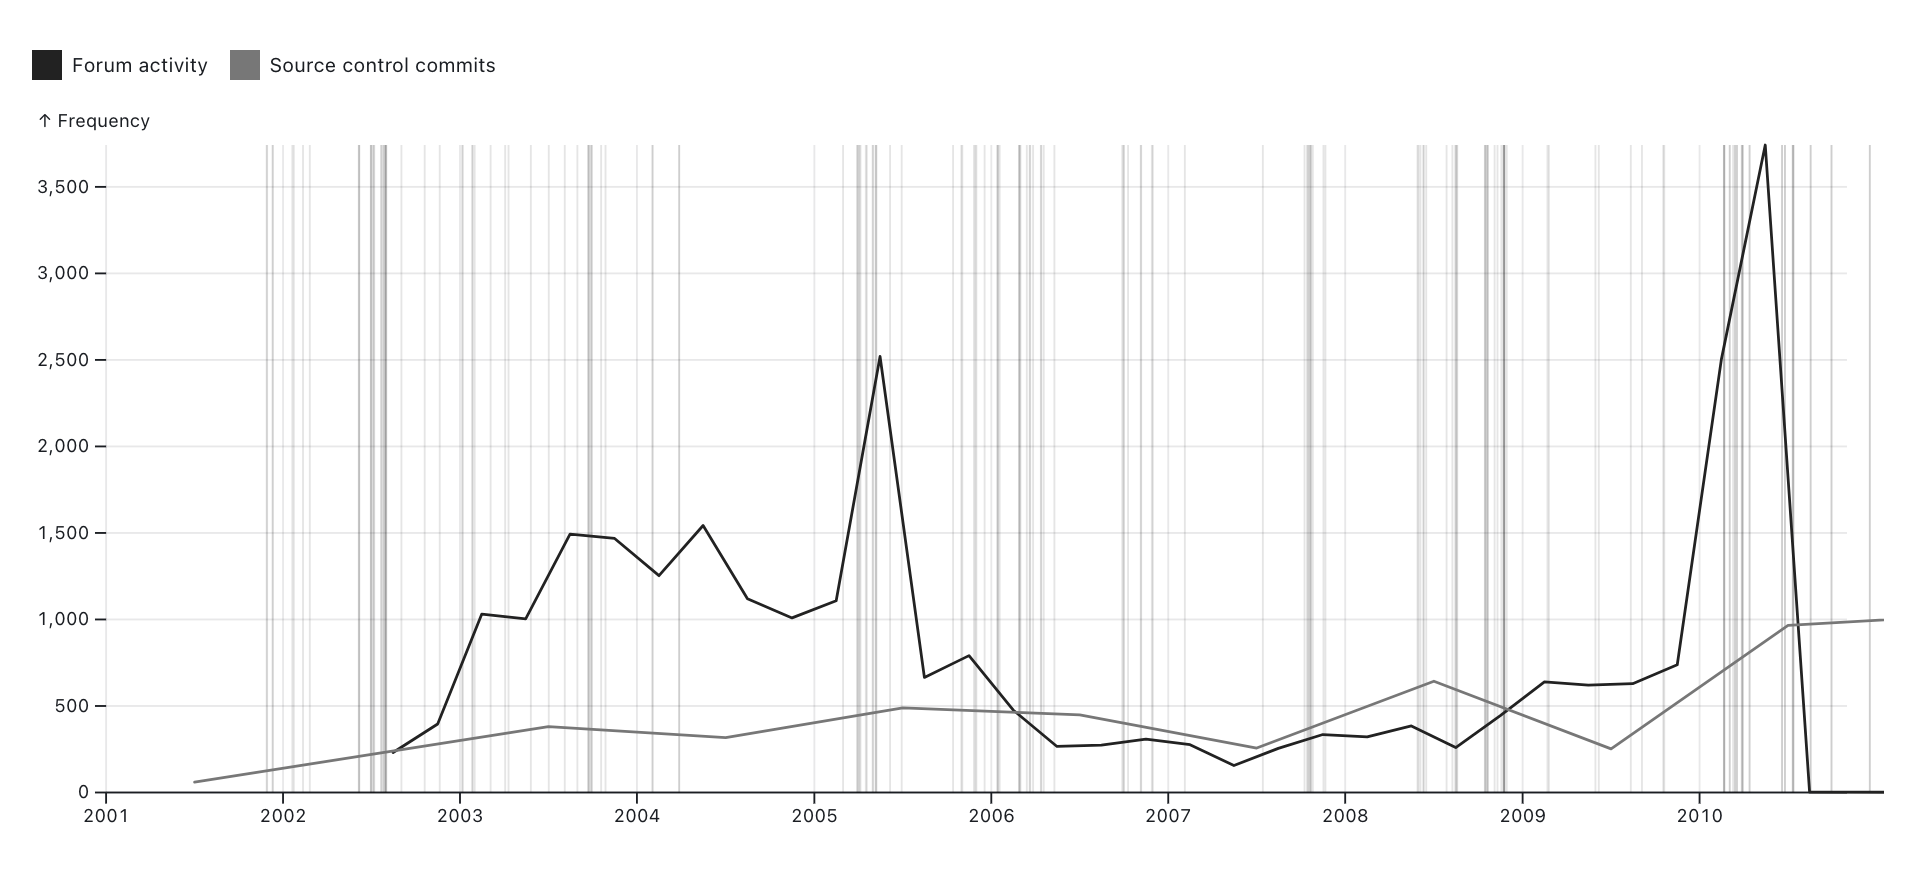
\includegraphics[width=1\textwidth]{images/figure-forum-git-activity.png} 

    \caption{Forum vs git activity vs releases (vertical lines)}
    \label{figure:forum-git-activity}  
  \end{figure}
      \end{block}
      \begin{block}{Furter research}
        \begin{itemize}
          \item Analyse corpus with Large Language Model (sentiment analysis, topic extraction)
          \item Investigate peaks in data
          \item Conduct a survay across most active contributors
          \item Setup interviews 
        \end{itemize}
      \end{block}

      \begin{block}{References}
        \printbibliography
      \end{block}
    \end{column}
    
  \end{columns}
\end{frame}
\end{document}